
\chapter{Derivatives}

This chapter covers the following ideas.  When you make your lesson
plan, it should cover all of these objectives.

% A list of objectives for the chapter
%\begin{enumerate}
%\item ...
%\end{enumerate}

\begin{enumerate}
\item Find limits and determine where functions of several variables
  are continuous.
\item Compute partial derivatives.  Use them to find tangent lines and
  tangent planes.
\item Be able to find the derivative of a function (as a matrix) and
  use it to find tangent planes.
\item Find derivatives of composite functions using the chain rule
  (matrix multiplication). In addition, find derivatives when
  constraints are in a problem.
\end{enumerate}

%%% Local Variables: 
%%% mode: latex
%%% TeX-master: "../multivariable-calculus"
%%% End: 
%$




\section{Limits and Continuity}
We start with some notation.  We will denote functions using $\vec f\colon
\mathbb{R}^n\to\mathbb{R}^m$ where $n$ is the number of inputs, and $m$
is the number of outputs.  We will use $\vec x$ to represent an input,
and $\vec y$ to represent an output.  For example, if $z=f(x,y)$, then
in vector notation we would write $\vec y=\vec f(\vec x)$, where $\vec
y=\langle z\rangle$ and $\vec x = \langle x,y\rangle$.  The parametric
surface $\vec r(u,v)=\langle x,y,z\rangle$ would be written as $\vec
f(\vec x)=\vec y$ where $\vec x = \langle u,v\rangle$ and $\vec
y=\langle x,y,z\rangle$.  Using this notation allows us to restate most
of the theorems of multivariable calculus using the exact same
notation as was learned in single variable calculus.

Recall that in first semester calculus, we defined the limit of a
function by saying that a function $y=f(x)$ has limit $L$ at $x=c$ if
for every $\epsilon>0$, there exists a $\delta>0$ such that if $0<|x-c|<\delta$, then
$|f(x)-L|<\epsilon$. The idea is that you can make the output value $y$ as
close to $L$ as you want (i.e., within $\epsilon$ of $L$) by requiring the
input values $x$ to be very close to $c$ (i.e., within $\delta$ of $c$).
This definition generalizes to all dimensions by placing vector
symbols above everything.  We say that a function $\vec y=\vec f(\vec
x)$ has limit $\vec L$ at $\vec x=\vec c$ if for every $\epsilon>0$, there
exists a $\delta>0$ such that if $0<|\vec x-\vec c|<\delta$, then $|\vec f(\vec
x)-\vec L|<\epsilon$. We interpret absolute values as distance (the square
root of the dot product). Learning to use the formal limit definition
to prove theorems about limits and derivatives will be deferred to a
course in real analysis, where an appropriate amount of time can be
spent on the topic. For now, the main idea is that a function has a
limit of $\vec L$ at $\vec c$ if the $\vec y$ values are close to
$\vec L$ for all $\vec x$ values close enough to $\vec c$.  We say
that a function is continuous at $\vec x=\vec c$ if the limit of the
function $\vec L$ equals $\vec f(\vec c)$ (i.e., $\lim_{\vec x \to \vec
  c}\vec f(\vec x)=\vec f(\vec c)$; we could just calculate the limit
by plugging in $\vec x=\vec c$).

The main difference between single-variable limits and multivariable
limits is that when there is only one input variable, you can study
limits from the left and limits from the right---those are the only
ways $x$ can move closer to $c$.  However, if there are more input
variables, then there are infinitely many ways to approach $\vec c$. A
limit exists at $\vec c$ if and only if the limit exists along
\emph{every} approach to $\vec c$.  For example, the function $f(x,y)
= \frac{x^2-y^2}{x^2+y^2}$ has a limit at every point in the plane
except at the origin because rational functions are continuous as long
as the denominator is nonzero.  We write $\ds
\lim_{(x,y)\to(a,b)}\frac{x^2-y^2}{x^2+y^2}=\frac{a^2-b^2}{a^2+b^2}$ as
long as $(a,b)\neq(0,0)$.  If $(a,b)=(0,0)$, then we will consider two
different ways of approaching the origin.  If we look at $(x,y)$
values on the $x$-axis, then we write $\ds
\lim_{\text{\tiny$\begin{array}{c} (x,y)\to(a,b)\\y=0
\end{array}$}} 
\frac{x^2-y^2}{x^2+y^2} = \lim_{x\to 0} \frac{x^2}{x^2}=1$.
Alternatively, if we look at $(x,y)$ values on the $y$-axis, then we
write 
$\ds \lim_{\text{\tiny$\begin{array}{c}
 (x,y)\to(a,b)\\x=0
\end{array}$}} \frac{x^2-y^2}{x^2+y^2} = \lim_{y\to 0}
\frac{-y^2}{y^2}=-1$. Hence we see that the limit is not the
same for different approaches.  In fact, if we only consider $(x,y)$
values on the line $y=mx$ for any $m$, then we write 
$\ds \lim_{\text{\tiny$\begin{array}{c}
 (x,y)\to(a,b)\\y=mx
\end{array}$}} \frac{x^2-y^2}{x^2+y^2} = \lim_{x\to 0}
\frac{x^2-(mx)^2}{x^2+(mx)^2}=\frac{1-m^2}{1+m^2}$, which is different
for each $m$. We say that the function $f$ has no limit (or the limit is undefined) at the
origin because the limit is not the same along different approaches. 

If a function has a limit, then the limit will be the same regardless
of the approach. In the functions below, the first does not have a
limit at the origin, the second does, and the third is discontinuous
along an entire curve $y=x^2$.

\begin{center}
\begin{tabular}{ccc}
\tikzsetfigurename{limits-}
\remake
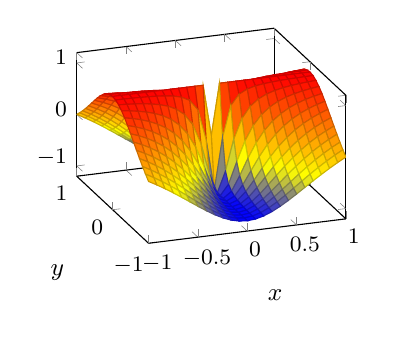
\begin{tikzpicture} 
  \begin{axis}[footnotesize, view/h=-20,xlabel=$x$,ylabel=$y$] 
   \addplot3[surf,domain=-1:1,y domain=-1:1] (x,y,{(x^2-y^2)/(x^2+y^2)}); 
\end{axis} 
\end{tikzpicture}&
\remake

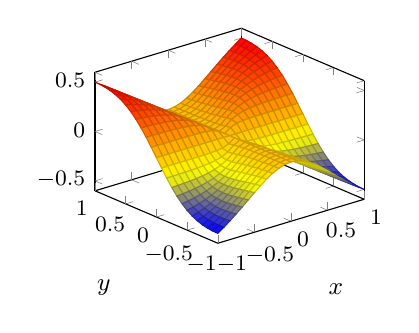
\begin{tikzpicture} 
  \begin{axis}[footnotesize, view/h=-40, xlabel=$x$,ylabel=$y$] 
    \addplot3[surf,domain=-1:1,y domain=-1:1] (x,y,{(x^2*y)/(x^2+y^2)}); 
 \end{axis} 
 \end{tikzpicture}&
 \remake
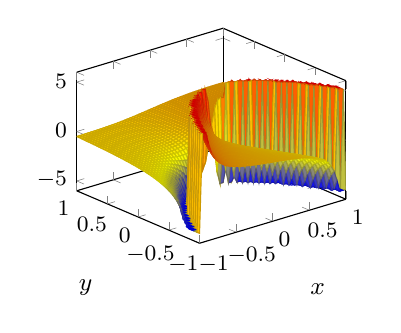
\begin{tikzpicture} 
  \begin{axis}[footnotesize, view/h=-40,
    xlabel=$x$,ylabel=$y$,restrict z to domain*=-5:5,samples=50] 
    \addplot3[surf,domain=-1:1,y domain=-1:1] (x,y,{(x)/(y+x^2)}); 
 \end{axis} 
 \end{tikzpicture}\\

$f(x,y)=\frac{x^2-y^2}{x^2+y^2}$ &
 $f(x,y)=\frac{x^2y}{x^2+y^2}$ &
 $f(x,y)=\frac{x}{x^2-y}$\\
\end{tabular}
\end{center}


\section{Partial Derivatives} 
If a function $f$ has only one input $x$, then the derivative is
defined to be $\ds \frac{d f}{dx} = \lim_{h\to 0}\frac{f(x+h)-f(x)}{h}$.
The derivative gives the best possible linear approximation to changes
in a function. This idea is represented by the equation $\Delta  y \approx
f^\prime(x)\Delta x$, or in differential form, we write $d y=f^\prime(x) dx$.  An
equation of a tangent line is found by noticing that a change in $y$
is approximately $y-f(c)$ when the change in $x$ is $x-c$, so the
differential form $dy=f^\prime dx$ becomes $(y-f(c))=f^\prime(c)(x-c)$.  I
repeat, the derivative gives the best possible linear approximation to
changes in a function.

If a function has more than one input variable, then division by the
vector $\vec h$ is not well-defined, so we run into a problem with
generalizing derivatives.  Instead, we start with partial derivatives,
which approximate change in the function if we hold all other
variables constant and just differentiate with respect to one
variable.  For the function $f(x,y)$, we define the partial derivative
of $f$ with respect to $x$ as $\ds f_x(x,y)=f_x = \frac{\partial f}{\partial x}=
\lim_{h\to 0}\frac{f(x+h,y)-f(x,y)}{h}$, and the partial derivative of
$f$ with respect to $y$ as $\ds f_y(x,y)=f_y =\frac{\partial f}{\partial y}=
\lim_{k\to 0}\frac{f(x,y+k)-f(x,y)}{k}$. Notice that $f_x$ computes a
limit as $y$ is held constant and we vary $x$. For
$f(x,y)=3x^2+4xy+\cos(xy)+y^3$, we obtain $f_x=6x+4y-y\sin(xy)+0$ and
$f_y=0+4x-x\sin(xy)+3y^2$. Partial derivatives are found by holding
all other variables constant, and then differentiating with respect to
the variable in question. Practice computing partial derivatives with
lots of functions. The homework should go very quickly, but this skill
needs plenty of practice so that partial differentiation is done
immediately.

Partial derivatives approximate change in a function as you vary only
one variable, hence a partial derivative gives slope in the direction
which is varied. For the function $z=f(x,y)$, $f_x$ is the slope of a
line tangent to the surface $z=f(x,y)$, where the tangent line is
parallel to the $xz$-plane. A direction vector for this line is
$\langle1,0,f_x\rangle$ (every increase in $x$ of 1 unit yields an
increase in the output $z$ of $f_x$ units, and $y$ does not change). 
Similarly $\langle0,1,f_y\rangle$ is a direction vector of a line
tangent to the surface, where the line is parallel to the $yz$-plane.
The cross product of these two vectors is $\vec n =
\langle-f_x,-f_y,1\rangle$, which is a normal vector for the tangent
plane to the surface. For the function $f(x,y)=9+x-y^2$ at
$(x,y)=(1,2)$, we have $f(x,y)=6$, $f_x(x,y) =1$, $f_y(x,y)=-2y$,
$f_x(1,2)=1$, and $f_y(1,2)=-4$. So a tangent line to the surface at
$(1,2,6)$ in the $x$ direction is $\vec r(t) = \langle1,0,1\rangle t+ 
\langle1,2,6\rangle$, in the $y$ direction is $\vec r(t) =
\langle0,1,-4\rangle t+  \langle1,2,6\rangle$, and an equation of the
tangent plane is $-1(x-1)+4(y-2)+1(z-6)=0$. The pictures below
illustrate these lines and planes 

\renewcommand{\mywidth}{1.3in}
\begin{center}
\begin{tabular}{ccc}
\includegraphics[width=\mywidth]{04-Derivatives/support/tan-1}&
\includegraphics[width=\mywidth]{04-Derivatives/support/tan-2}&
\includegraphics[width=\mywidth]{04-Derivatives/support/tan-3}
\\
$y$ is constant, $\vec v = \langle1,0,f_x\rangle$ &
$x$ is constant, $\vec v = \langle0,1,f_y\rangle$ &
Tangent plane $n=\langle-f_x,-f_y,1\rangle$
\end{tabular}
\end{center}



For the parametric surface $\vec r(u,v)=\langle u,v,9+u-v^2\rangle$, we
compute $\vec r_u = \langle1,0,1\rangle$ and $\vec r_v =
\langle0,1,-2v\rangle$, which are direction vectors for tangent lines
to the surface (notice they are the same vectors as in the previous
example).  At the point $(u,v)=(1,2)$, the tangent lines and tangent
plane are exactly the same as those for the function
$z=f(x,y)=9+x-y^2$. 

Since a partial derivative is a function itself, you can take
derivatives of a partial derivative as well, giving what is called
higher order partials.  For the function $f(x,y,z)=x^2+4xy^2-yz^3$, we
have $f_x=2x+4y^2, f_y=8xy-z^3, f_z=-3yz^2$, and so we obtain the
following second order partial derivatives $
\frac{\partial}{\partial x}f_x = f_{xx} = 2,
\frac{\partial}{\partial y}f_x = f_{xy} = 8y,
\frac{\partial}{\partial z}f_x = f_{xz} = 0,
\frac{\partial}{\partial x}f_y = f_{yx} = 8y,
\frac{\partial}{\partial y}f_y = f_{yy} = 8x,
\frac{\partial}{\partial z}f_y = f_{yz} = -3z^2, 
\frac{\partial}{\partial x}f_z = f_{zx} = 0, 
\frac{\partial}{\partial y}f_z = f_{zy} = -3z^2, 
\frac{\partial}{\partial z}f_z = f_{zz} = -6z.$
Notice that $f_{xy}=f_{yx}, f_{xz}=f_{zx}$, and $f_{zy}=f_{yz}$. As
long as a function is two times continuously differentiable, then
second order partial derivatives using the same variables but in a
different order will always be the same. This fact will get used
periodically throughout the class.

\section{The Derivative} 
The derivative of a function $\vec f:\mathbb{R}^n\to\mathbb{R}^m$ is an
$m\times n$ matrix, notated as $D\vec f(\vec x)$, where the columns of the
matrix are the partial derivatives of the function with respect to
each input variable (the first column is the partial derivative with
respect to the first variable, and so on). Some people call this
derivative the ``total'' derivative instead of the derivative, to
emphasize that the ``total'' derivative combines the ``partial''
derivatives into a matrix. This matrix is also called the Jacobian
matrix (or sometimes simply the Jacobian) of the function.  This
definition of the derivative gives the best possible linear
approximation to changes in a function. A full course in linear
algebra is needed to fully understand the significance of this
statement, however we can use the derivative as a matrix to simplify a
lot of our work in multivariable calculus.

Some examples of functions and their derivatives are in Table~\ref{tab:derivatives}. When the
output dimension of a function is one, then the matrix has only one
row. In this case, we often consider it as a row vector and the
derivative is called the gradient of $f$ and written $\nabla f$.  

\begin{table}[h]
  \centering
    \begin{tabular}{ll}\toprule
Function&Derivative\\ \midrule
{$f(x)=x^2$}& {$Df(x) = \begin{bmatrix}2x\end{bmatrix} $}\\ 
{$\vec r(t) = \langle3\cos(t),2\sin(t)\rangle$}&  {$D\vec r(t) =
\begin{bmatrix}-3\sin t\\ 2\cos t\end{bmatrix} $}\\ 
{$\vec r(t) = \langle\cos(t),\sin(t),t\rangle$}&  {$D\vec r(t) =
\begin{bmatrix}-\sin t \\ \cos t \\ 1\end{bmatrix} $}\\ 
{$f(x,y)=9-x^2-y^2$}&  {$Df(x,y) =\nabla f(x,y) = \begin{bmatrix}-2x &
-2y\end{bmatrix} $}\\ 
{$f(x,y,z)=x^2+y+xz^2$}&  {$Df(x,y,z) = \nabla f(x,y,z) =
\begin{bmatrix}2x+z^2 & 1 &2xz\end{bmatrix} $}\\ 
{$\vec F(x,y)=\langle-y,x\rangle$}&  {$D\vec F(x,y) =
\begin{bmatrix}0&-1\\ 1&0\end{bmatrix} $}\\ 
{$\vec F(r,\theta,z)=\langle r\cos\theta,r\sin\theta,z\rangle$}&  {$D\vec F(r,\theta,z) = 
\begin{bmatrix}
\cos \theta &-r\sin\theta&0\\ 
\sin\theta&r\cos\theta&0\\ 
0&0&1
\end{bmatrix} $}\\ 
{$\vec r (u,v)=\langle u,v,9-u^2-v^2\rangle$}&  {$D\vec r(u,v) =
\begin{bmatrix}1&0\\ 0&1\\ -2u&-2v\end{bmatrix} $}\\ 
      \\\bottomrule
    \end{tabular}

  \caption{Example derivatives}
  \label{tab:derivatives}
\end{table}

To emphasize that the derivative is the best possible linear
approximation to changes in a function, replace $f^\prime$ in the single
variable equation $dy=f^\prime dx$ with the derivative $D\vec f(\vec x)$ to
obtain $d\vec y =D\vec f(\vec x)d\vec x$ ($d[\text{outputs}]=Df
d[\text{inputs}]$).  For a function $z=f(x,y)$ we obtain
$dz=Df(x,y)\begin{bmatrix}dx\\dy\end{bmatrix} =
\begin{bmatrix}f_x&f_y\end{bmatrix}\begin{bmatrix}dx\\dy\end{bmatrix}
= f_xdx+f_ydy$ using matrix multiplication. To get an equation of a
tangent plane to a surface at $(a,b,f(a,b))$, we let $dz=z-f(a,b),
dx=x-a,dy=y-b$, and then obtain $z-f(a,b) =
\begin{bmatrix}f_x&f_y\end{bmatrix}\begin{bmatrix}x-a\\y-b\end{bmatrix}=f_x(a,b)
(x-a)+f_y(a,b)(y-b)$. This is equivalent to  $-f_x(a,b)
(x-a)-f_y(a,b)(y-b)+z-f(a,b)=0$, which is the equation of a plane with
normal vector $\vec n=\langle-f_x,-f_y,1\rangle$, which we already
obtained in the partial derivatives section. For the function
$f(x,y)=9+x-y^2$ at $(x,y)=(1,2)$, an equation of the tangent plane is
simply  $z-6 =
\begin{bmatrix}1&-4\end{bmatrix}\begin{bmatrix}x-1\\y-2\end{bmatrix}$. 
This version of finding tangent planes generalizes to all dimensions
and gives the ``tangent space.''

This optional paragraph explains why the definition of the derivative
above makes sense. Since division by $\vec h$ is not defined if $\vec
h$ is a vector and not a number, we modify the definition of the
derivative to define the derivative of a function in general. The
definition of the derivative when written using the formal definition
of a limit requires that we examine the inequality
$|\frac{f(x+h)-f(x)}{h} - f^\prime(x)|<\epsilon$.  Multiply both sides by $|h|$
and obtain $|f(x+h)-f(x) - f^\prime(x)h|<\epsilon|h|$. The derivative of a
function $\vec f:\mathbb{R}^n\to\mathbb{R}^m$ gives the best possible
linear approximation to changes in the function. A course in linear
algebra will show you that this means the derivative can be
represented by a matrix, and then the equation $|\vec f(\vec x+\vec
h)-\vec f(\vec x) - D\vec f(\vec x)\vec h|<\epsilon|\vec h|$ shows that
$D\vec f(\vec x)$ must be able to multiply on the right by vectors of
size $n$ (hence it has $n$ columns), and the product $D\vec f(\vec
x)\vec h$ must give a vector with $m$ components (hence the matrix has
$m$ rows). By considering the vector $\vec h =
\langle h_1,0,\ldots,0\rangle$, it can be shown that the first column of
$D\vec f(\vec x)$ equals the partial derivative of $\vec f$ with
respect to the first variable. 
 
\section{The Chain Rule}
For multivariable functions, we can form the composition $\vec f\circ \vec
g$ of two functions $\vec f:\mathbb{R}^n\to \mathbb{R}^m$ and $\vec
g:\mathbb{R}^p\to \mathbb{R}^n$ provided that output dimension of $\vec
g$ is the same as the input dimension of $\vec f$.  The composition
$\vec f(\vec g(\vec x))$ essentially asks us to put into the function
$\vec g$ a vector $\vec x$ of size $p$, which will give us a vector
$\vec g(\vec x)$ of size $n$.  Since this is the dimension of the
domain of $\vec f$, then we can put $\vec g(\vec x)$ into the function
$\vec f$, and we get a vector $\vec f(\vec g(\vec x))$ of size $m$.
For example, if $f(x,y)=x^2-y$ and $\vec
g(r,s,t)=\langle3r+4s,t^2-r\rangle$, then $f(\vec g(r,s,t)) =
f(3r+4s,t^2-r) = (3r+4s)^2-(t^2-r)$.

Recall from first semester calculus the chain rule: {$(f\circ g)^\prime(x) =
  f^\prime(g(x))g^\prime(x)$} (the derivative of the outside function multiplied
by the derivative of the inside function). The high-dimensional
version of the chain rule is exactly the same, namely {$D(\vec f\circ \vec
  g)(\vec x) = D\vec f(\vec g(\vec x))D\vec g(\vec x)$}, and a proof
is essentially the same (but we will leave this to another course).
The product is matrix multiplication. Most textbooks explain a rule
for remembering the multiplications involved in the chain rule, but
these are just ways of organizing matrix multiplication without
referring to a matrix.

We now look at a few examples. Suppose the temperature at each point
in the plane is given by {$f(x,y) = 9-x^2-y^2$}.  A particle moving
through the plane along the curve $x=t+1, y=t^2$ will have a
temperature given by $f(r(t)) = f(t+1,t^2) = 9-(t+1)^2-(t^2)^2$.  We
will find the rate of change of the temperature of the particle as it
moves through the plane, which we call {$\frac{df}{dt}$}. Let's give
the path $x=t+1, y=t^2$ a name, for example let {$\vec r(t) =
  \langle t+1,t^2\rangle$}.  Then the composition {$f(\vec r(t))$} is
the temperature of the particle at any time {$t$}.  Hence, we are
really trying to compute {$\frac{d(f\circ r)}{dt}$}, which gets tedious to
write, so most people abbreviate it with {$\frac{df}{dt}$}, even
though there are no {$t$} variables in the definition of {$f(x,y)$}.  The
chain rule says that I can compute this value by finding {$Df(x,y)$}
and {$D\vec r(t)$}, evaluating {$Df(x,y)$} at {$\vec r(t)$} (which
gives me {$Df(\vec r(t))$}), and then multiplying the matrices
together. The calculations are $Df(x,y) = \begin{bmatrix}-2x &
  -2y\end{bmatrix}$ and $D\vec r(t) = \begin{bmatrix}1\\
  2t\end{bmatrix}$, so $Df(\vec r(t)) =
\begin{bmatrix}-2(t+1) & -2(t^2)\end{bmatrix}$. We then calculate 
$$D(f\circ \vec r)(t) = Df(\vec r(t))D\vec r(t)=\begin{bmatrix}-2(t+1) &
  -2(t^2)\end{bmatrix} \begin{bmatrix}1\\ 2t\end{bmatrix}=
(-2(t+1))(1) + (-2(t^2))(2t).$$ We can also do this by just replacing
{$x$} and {$y$} with what they are in terms of $t$, and then
differentiating $f(r(t)) = 9-(t+1)^2-(t^2)^2$.  This second approach
may at first seem easier, but the first approach becomes essential
when you want to do implicit differentiation and high-dimensional
calculus.  To summarize the two-variable case, we just developed the
formula $\ds \frac{df}{dt}=\begin{bmatrix}f_x &
  f_y\end{bmatrix} \begin{bmatrix}x_t\\ y_t\end{bmatrix}=f_xx_t+f_yy_t
= \frac{\partial f}{\partial x}\frac{dx}{dt}+\frac{\partial f}{\partial y}\frac{dy}{dt}$.

For $f(x,y,z) = 3xy+z^2$ and $x=2u+v,y=u-v,z=uv$, we can compute both
$\frac{\partial f}{\partial u}$ and $\frac{\partial f}{\partial v}$ using the chain rule.  Again,
let's name the function $x=2u+v,y=u-v,z=uv$, using something like $\vec
r(u,v) = \langle2u+v,u-v,uv\rangle$.  Then the derivative $D(f\circ \vec
r)$ is found by multiplying
\begin{align*}
D(f\circ \vec r)(u,v) = Df(x,y,z)D\vec r(u,v)
&=\begin{bmatrix}f_x & f_y &f_z \end{bmatrix} \begin{bmatrix}x_u&x_v\\
y_u&y_v\\z_u&z_v\end{bmatrix} \\
&= \begin{bmatrix}3y & 3x &2z \end{bmatrix} \begin{bmatrix}2&1\\
1&-1\\v&u\end{bmatrix} \\
&=\begin{bmatrix}(3y)(2) + (3x)(1)+(2z)(v) & (3y)(1) + (3x)(-1)
+(2z)(u)  \end{bmatrix}.
\end{align*} 
Replacing $x,y,z$ with what they are in terms of $u$ and $v$ gives
$$D(f\circ \vec r)(u,v)=\begin{bmatrix}6(u-v) + 3(2u+v)+2uv^2 & 3(u-v)
-3(2u+v) + 2u^2v  \end{bmatrix}.$$ The first column of the matrix is
the partial with respect to $u$, so $\frac{\partial f}{\partial u} = 6(u-v) +
3(2u+v)+2uv^2$ and the second column gives $\frac{\partial f}{\partial v} = 3(u-v)
-3(2u+v) + 2u^2v$.
We just developed the general formula 
$$D(f\circ \vec r)(u,v)=\begin{bmatrix}f_u & f_v 
\end{bmatrix}=\begin{bmatrix}f_xx_u + f_yy_u+f_zz_u & f_xx_v +
f_yy_v+f_zz_v  \end{bmatrix}.$$

For an equation of the form $y^2x+x-xy=1$, we learned how to calculate
$\frac{dy}{dx}$ implicitly in first-semester calculus.  We now learn a
quick method using high-dimensional calculus. Let $f(x,y) = y^2x+x-xy$
and $\vec r(x) = \langle x,y(x)\rangle$ be a parametrization of the
curve. Composition shows that $f(\vec r(x))=1$, a constant, so the
derivative is zero.  We compute this derivative: $D(f\circ r)(x) = Df(\vec
r(x))D\vec
r(x)=\begin{bmatrix}f_x& f_y\end{bmatrix}\begin{bmatrix}1 \\
  \frac{dy}{dx}\end{bmatrix}$.  Matrix multiplication gives $f_x+f_y
\frac{dy}{dx}=0$ so $\frac{dy}{dx} = -\frac{f_x}{f_y} =
-\frac{y^2+1-y}{2xy-x}$.  This idea can be generalized to do implicit
differentiation in any setting. This illustrates an important
idea. Some problems become easier to solve in higher dimensions.
Sometimes the only solution to a problem is found by looking at the
problem in a higher dimensional space where there are more tools
available.



\section{Partial Derivatives with constrained variables}
When you have many variables in a problem, it is important to specify
which are independent and which are dependent on another
variable. Your choice could significantly change the values of the
partial derivatives.  When there are many variables in a problem, we
will use the notation {$\displaystyle\left(\frac{\partial w}{\partial
      x}\right)_{y,z}$} to signify that {$x,y,z$} are the independent
variables and the other variables all depend on {$x,y,z$}.  If the
variables that you see in the problem are $x,y,z$, and $t$, and $w$ is
a function of all of these variables, then often it is helpful to
create a diagram of the form $\begin{bmatrix}x\\y\\z\end{bmatrix}\to
\begin{bmatrix}x\\y\\z\\t\end{bmatrix}\to \begin{bmatrix}w\end{bmatrix}$
to remind yourself how the variables relate, namely that $t$ depends
on the other variables.  Then you can use the chain rule to find the
partials of {$w$} with respect to any variable you wish.

For example, let $w=x^2-y^2+z-\sin(t)$ and $x-y^2+3z=5t$ (the equation
$x-y^2+3z=5t$ is called a constraint because it puts a limitation on
the values you can pick for $x,y,z,$ and $t$).  Then
$\displaystyle\left(\frac{\partial w}{\partial x}\right)_{y,z}$ is found in one of
two ways.  The first approach (which you can use for the homework and
exams) is to replace $t$ with what it is in terms of $x,y,$ and $z$,
and then take the partial with respect to $x$.  This is by far the
quickest route, if you are just after a number.  In this case we get
$t=(x-y^2+3z)/5$ and so $w = x^2-y^2+z-\sin((x-y^2+3z)/5)$.  Then
$\displaystyle\left(\frac{\partial w}{\partial x}\right)_{y,z} =
2x-0+0-\cos((x-y^2+3z)/5)\cdot \frac{1}{5}$.

The other option involves a theoretical understanding.  Start by
making the diagram $\begin{bmatrix}x\\y\\z\end{bmatrix}\to
\begin{bmatrix}x\\y\\z\\t\end{bmatrix}\to
\begin{bmatrix}w\end{bmatrix}$. Notice that $t$ is the dependent
variable, so we have $t=\frac{1}{5}(x-y^2+3z)$. This is a composite
function, and the derivative is
$$Dw(x,y,z)=\begin{bmatrix}w_x&w_y&w_z&w_t\end{bmatrix}\begin{bmatrix}x_x&x_y&x_z\\y_x&y_y&y_z\\z_x&z_y&z_z\\t_x&t_y&t_z\end{bmatrix}
= \begin{bmatrix}2x&-2y&1&-\cos
t\end{bmatrix}\begin{bmatrix}1&0&0\\0&1&0\\0&0&1\\1/5&-2y/5&3/5\end{bmatrix}.$$
Since I am only after $\displaystyle\left(\frac{\partial w}{\partial
x}\right)_{y,z}$, I want the partial with respect to $x$ which means
the first column of $Dw(x,y,z)$ or $2x-\frac{1}{5}\cos(t) =
2x-\frac{1}{5}\cos(\frac{1}{5}(x-y^2+3z))$.  The second column would
give $\displaystyle\left(\frac{\partial w}{\partial y}\right)_{x,z}$, and the third
column $\displaystyle\left(\frac{\partial w}{\partial z}\right)_{x,y}$. If on the
other hand I were asked to compute
$\displaystyle\left(\frac{\partial w}{\partial z}\right)_{y,t}$, then $x=5t-3z+y^2$
and so \note{Check these matrices to make sure they are correct.}
$$Dw(y,z,t)=\begin{bmatrix}w_x&w_y&w_z&w_t\end{bmatrix}\begin{bmatrix}x_y&x_z&x_t\\y_y&y_z&y_y\\z_y&z_z&z_y\\t_y&t_z&t_y\end{bmatrix}
= \begin{bmatrix}2x&-2y&1&-\cos
t\end{bmatrix}\begin{bmatrix}2y&-3&5\\1&0&0\\0&1&0\\0&0&1\end{bmatrix},$$
which means that $\displaystyle\left(\frac{\partial w}{\partial z}\right)_{y,t}=
2(x)(-3)+(1)(1)= -6(5t-3z+y^2)+1$ is the second column of $Dw(y,z,t)$. 

As a last example, if $w=x^2+y+z^2$ and $x^2+y=z^3$, then we can
compute $\displaystyle\left(\frac{\partial w}{\partial x}\right)_{z}$ by writing
$y=z^3-x^2$ and $w=x^2+(z^3-x^2)+z^2 = z^3-z^2$.  The partial with
respect to $x$ when $y$ is dependent is hence 0.  On the other hand,
we can compute $\displaystyle\left(\frac{\partial w}{\partial x}\right)_{y}$ by
writing $z=\sqrt[3]{x^2+y}$ and $w=x^2+y+(\sqrt[3]{x^2+y})^2$. The
derivative of this with respect to $x$ is
$2x+\frac{2}{3}(x^2+y)^{-1/3}2x $, which is not zero. Specifying which
variables depend on which makes a difference when taking derivatives
where constraints are present.




%%% Local Variables: 
%%% mode: latex
%%% TeX-master: "../multivariable-calculus"
%%% End: 





